\chapter{Experimenton and Results}


\section{Introduction}
Over the course of this work it was concluded that the radar data was not appropriate for Map Building or for localization using \ac{AMCL}. However it was noted that the radar was quicker   at detecting different types of obstacles. In the following subsections we will describe how a differential drive robot usually is able to avoid  said obstacles. 
First a description of what is obstacle avoidance is and how it  works, the robots kinematic model, then the description of how he perceives the world around him (configuration space), then how the robot plans around said world in a good fashion.
\section{Obstacle avoidance}
 Obstacle avoidance is a major subject in robotics, failure in this systems may result in crashes that have catastrophic consequences such as hardware being badly damaged or completely nonfunctional. This problem is usually separated into two categories local path planning and global path planning. 
 Global methods assume the environment is completely known a priori and can therefore compute an optimal safe path  around static obstacles using a variety of different strategies. This models prove to be very reliable for static environments. However this models are usually computational expensive which lead to very slow update times. For fast changing environments such as is in the case for highly populated indoor scenarios they prove to be insufficient. 
 To improve the quality of navigation capabilities, local path planning techniques are added to improve the responsiveness of the robot. This techniques have a much faster update time  since they use a smaller version of the world around them. However this type of approaches have trouble with local minimum cases where the robot gets stuck (for example the U-shape case).
\subsection{Global Methods}
Path planning is crucial for the robot to handle safe trajectory around obstacles. In this work the information regarding this obstacles is based on a grid map built by \ac{SLAM} and new observations retrieved by the robot's sensors.  Planning an optimal safe path can be done using a wide variety of methods like Visibility Graphs, Generalized Voroin Diagram, and \ac{PRM} \cite{globalmethods}. However for in this work we will use the \ac{PRM} method. This method samples its environment and creates a occupancy graph. Then by inserting the initial position and the goal position the path can be computed using dijaktra or A* or Rapidly exploring Random Trees search algorithms . However, the \ac{ROS} navigation packages only use the first two so  we will only focus on this ones.


\subsubsection{Dijaktra algorithm}
Assuming we have an occupancy map we can now start to explain how does a robot compute the shortest path between the starting position and the end goal. Edsgar W. Dijkstra proposed an algorithm that solves this problem for a number of nodes, in our case we have cells on an occupancy grid map. Assuming with each cell costs the same then the shortest path can be calculated doing the following algorithm described in Figure \ref{fig:dalg}. 
\begin{figure}[h] 
\centerline{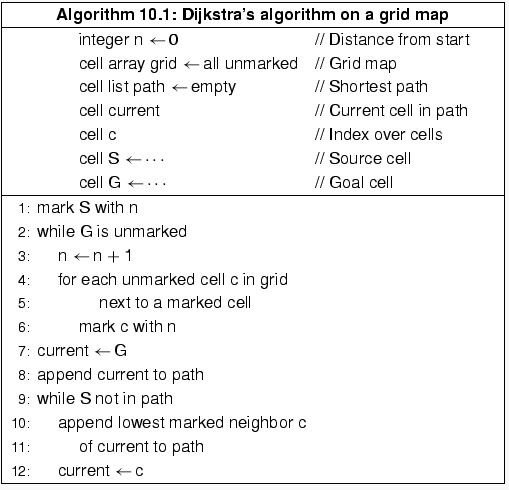
\includegraphics [width=0.7 \textwidth]{imgs/chapter5/Dalg.png}}
\caption{(taken form \cite{Ben-Ari2018})}
\label{fig:dalg}
\end{figure}
Each cell is numbered with the number of steps it needs to get to the starting position. This continues until we reach the goal cell and we get the minimum path to reach it. However if we have a map with cells that have variable cost in the algorithm above we do not iterate $n$ with plus one, but with the cell cost. This makes it so for this case that  shortest path geometrically may not be the shortest path when the costs are taken into account.

\subsubsection{A* algorithm}
In the previous case we search for cells in all directions, however there is a more efficient way of doing it by adding more information. The A* algorithm takes into account an extra \textit{heuristic function} to that gives a preferred direction for the search. Not only does it take into account the cell cost but another value that corresponds to a given direction to be doing in  the search. The function can be shown as:
\begin{equation}
    f(x,y)=g(x,y) + h(x,y)
\end{equation}
\subsection{Local Methods}
In contrast to global path planning in where a large portion of the environment is generally assumed to be true, local methods take in to account a partial world view for the motion planning capabilities. In other words, local path planning determines the motion of the robot taking into account the global plan provided by the global methods described earlier.
The most popular of this type of methods are \cite{inbookdwa}:
%cite this
\begin{itemize}
    \item Dynamic Window Approach
    \item Trajectory Rollout
    \item Elastic Band
    \item Timed elastic band
    \item VFH+
\end{itemize}
For our case study we will only explore the first two that are already integrated in ROS.
\subsubsection*{Trajectory Rollout}
The Trajectory Rollout  the most standard approach when it comes to local path planning in \ac{ROS}. It outputs  rotational and translational velocity by generating multiple trajectories for different types of velocity sample search space and choosing the best one. The algorithm goes as follows \cite{inbookdwa}:
\begin{itemize}
    \item Start with a set of velocities pairs $\{R_{vR_x},R_{ \omega_z} \}$ that are obtainable by the robot.
    \item Genarate in the form of arcs the projected trajectories obtained using the previous velocity sample space.
    \item Dismiss velocities that result in the robot colliding with an object in a given time frame. With this we are left of a subset of admissible velocities $V_a=R_{vR_a},R_{ \omega_a}$ in which:
    \begin{equation}
         V_a=R_{vR_a},R_{ \omega_a} \iff \begin{cases}
    R_{vR_x} & 	\leq \sqrt{2*dist(R_{vR_x},R_{ \omega_z})*R_{\dot{v}_{xb}}}.\\
    R_{ \omega_z}  &  	\leq \sqrt{2*dist(R_{vR_x},R_{ \omega_z})*R_{\dot{\omega}_{zb}}}.
  \end{cases}
    \end{equation}
    Where $R_{\dot{v}_{xb}}$ and $R_{\dot{\omega}_{zb}}$ are the braking accelerations of the robot and $dist$ the distance to the closest obstacle on the trajectory.
    
    
    \item Dismiss velocities that don't respect the robot's acceleration limits in a given simulated time frame. With this we are left with a subset of velocities called dynamic window $V_d=R_{vR_d},R_{ \omega_d}$  in which:
    \begin{equation}
         V_d=R_{vR_d},R_{ \omega_d} \iff \begin{cases}
    R_{vR_x} & 	\in [R_{v_a}-R_{\dot{vR}_{x}}*t,R_{v_a} + R_{\dot{vR}_{x}}*t].\\
    R_{\omega_z} & 	\in [R_{ \omega_a}-R_{\dot{\omega}_{z}}*t,R_{\omega_a}+R_{\dot{\omega}_{z}}*t].\\
  \end{cases}
    \end{equation}
    \item Finally we choose  the most optimal trajectory and in consequence velocity pair taking into account a given objective cost function.
    The cost function used to evaluate a trajectory in the \ac{ROS} navigation stack local planners is given by:
    \begin{align*}
            \textbf{cost} = &
       \texttt{pdist\_scale} * \textbf{path\_dist}
       + \texttt{gdist\_scale} * \textbf{goal\_dist}\\
       &+\texttt{occdist\_scale} * \textbf{maxobscost} 
    \end{align*}
    
    Where \textbf{path\_dist} is the distance from the endpoint of the trajectory to the global path in map cells, \textbf{goal\_dist} is the distance from the endpoint of the trajectory to the local goal in map cells, and \textbf{maxobscost} is equal to the \textbf{maximum obstacle cost} (given by the local costmap) of all the points along the trajectory.
    \end{itemize}
%%GARBAGE

\subsection{Differential drive robots kinematic model}
For differential drive robots 
For a differential drive robot the position he is in can be best described by a simple triplet $(x,y,\theta)$. This position is relative to usually a  global coordinate frame. 
\subsection{Map Representation}



There are two ways in which the navigation stack deals with obstacle avoidance. One way is to plan around the obstacle using the global planner if the obstacle is said on the .
The motion controller will take into account this plan. 










The dynamic path-planning problem consists in finding a suitable plan for each new configuration of the environment by re computing a collision free path using the new information available at each time step

\section{Introduction}
With the configuration described in the previous section we can now start to experiment with the robotic platform to do certain navigation tasks. In this part we propose various experiments that try to evaluate the  performance of the \ac{FMCW} \ac{RADAR} as an alternative or support to the \ac{LiDAR} as an obstacle detector for indoor navigation.
\section {Experiment 2}
In this following test we want to answer two things: (1) Is the robot able to avoid people that obstruct its pre planned path only using the  \ac{FMCW} radar as an obstacle detector, and (2) if in this case it is also able to clear previously obstructed spaces (by the person in this case) by ray tracing its environment. This last requirement may provide to be difficult to get since the radar point cloud is less dense than the 2D laser range finder.
\subsection{Experimental Setup}
The robot starting position and goal were set the same as the last test, however in this case a single person was instructed to actively obstruct the robot's forward movement until the robot reaches its first goal. After reaching it the person is removed from the environment  and the robot is  instantaneously given a second goal which in this case is its the starting position. 
\subsubsection{Results}
\subsubsection{Laser}
As expected the robot was able to detect and avoid the person in all 5 cases. However it should be noted that in one of this cases the robot tried to avoid it by going through an obstructed space due to a missed detection. This lead to collision. The robot was also able to clear the previously obstructed spaces, getting to the starting position without avoiding past marked obstacles.
\subsection{Radar}
The radar was also able to detect the obstructing person and managed to plan around it in all cases. Since the radar cloud is less dense, clearing marked obstacles was slower than in the \ac{LiDAR} case. However this did not impact the overall performance of the navigation task in a significant way since it still had 
\subsection{Comments}
 The radar was also able to perform 
obstacle avoidance of dynamic obstacles (in this case a person that continuously obstructed its path at 5 different times in the same environment which may suggest the use of \ac{RADAR} as an alternate sensory unit over the \ac{LiDAR}.
\section {Experiment 3}
Over the course of this work the \ac{FMCW} radar has shown to have better performance at detecting certain indoor objects than the 2D \ac{LiDAR}. This means that there might be situations where using it for obstacle avoidance produce better results for indoor navigation tasks. To demonstrate this a test was devised in a controlled environment that compares the performance of each sensor for different types of obstacles, in this case two types of chairs, a garbage bin, a low height box, a transparent acrylic tube and finally a robot (in this case another tutlebot2).  We also try to use the fusion of both sensors that in theory should produce the best results.


To ensure the experiment is done in a controlled way the scenario shown in Figure \ref{fig:cenario} was constructed. 
\begin{figure}[ht!] 
    \begin{minipage}[b]{.49\linewidth}
        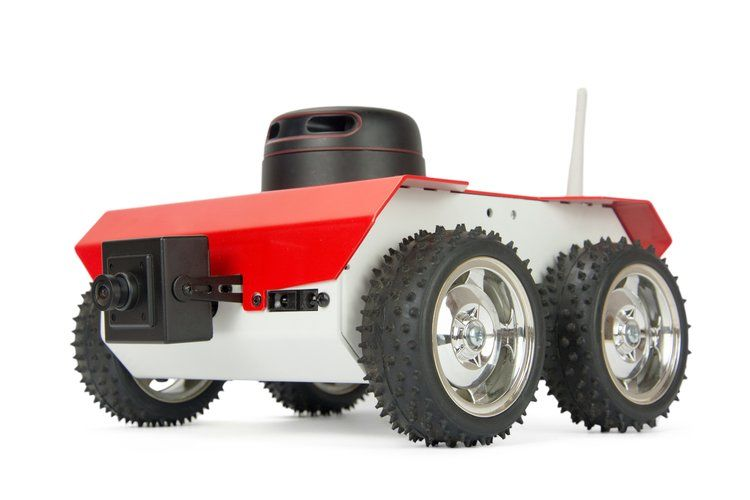
\includegraphics[height=5cm,width=\linewidth]{imgs/chapter2/robot1.jpg}
        \subcaption{Scenerio Foto \cite{robot1}}
        \label{fig:cenario}
    \end{minipage}
    \begin{minipage}[b]{.49\linewidth}
        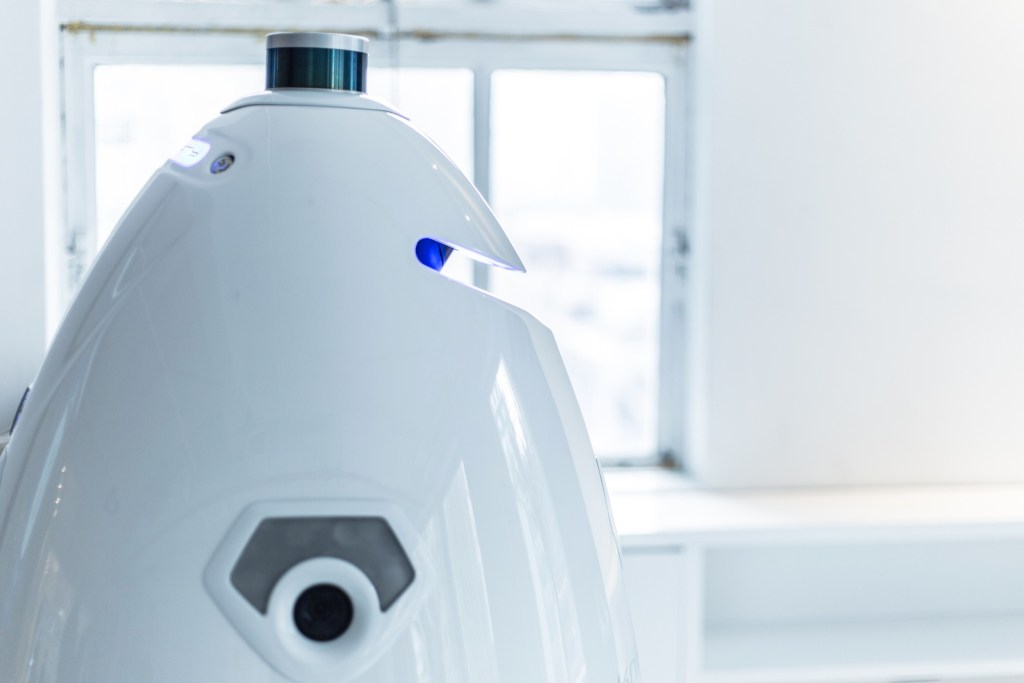
\includegraphics[height=5cm,width=\linewidth]{imgs/chapter2/robot2.jpg}
        \subcaption{Map pgm}
        \label{fig:map}
    \end{minipage}
    \caption{Different robots using \ac{LiDAR}}
    \label{fig:setup}
\end{figure}
This is a 4 by 4 meter squared box with 1 meter high walls with the addition of a half a meter wall in length in the middle. This type of environment optimizes the robots localization system (\ac{AMCL}) as well as make sure we only concentrate with one specific object at a time. Using a \ac{SLAM} package developed here at \ac{IRIS} a map is first created (Figure \ref{fig:map}) that will later be used for localization purposes.
\subsection{Experimental setup}
With the described scenario we setup the robots goal to make 5 loops between 2 goals, positioning in between the route an obstacle as illustrated in  figure X. If the obstacle detection system fails then the robot should collide with said object, if it succeeds the robot should go around the object leaving in between a relatively safe distance. The test was made using the \ac{FMCW} radar, the 2D \ac{LiDAR}, and the fusion of both for different types of objects. The  navigation data was recorded in a rosbag file in order to be analyzed later.

The list of objects used as obstacles are displayed in Fig. \ref{fig:obstacles}.

\begin{figure}[h!]
  \centering
  \begin{subfigure}[b]{0.3\linewidth}
    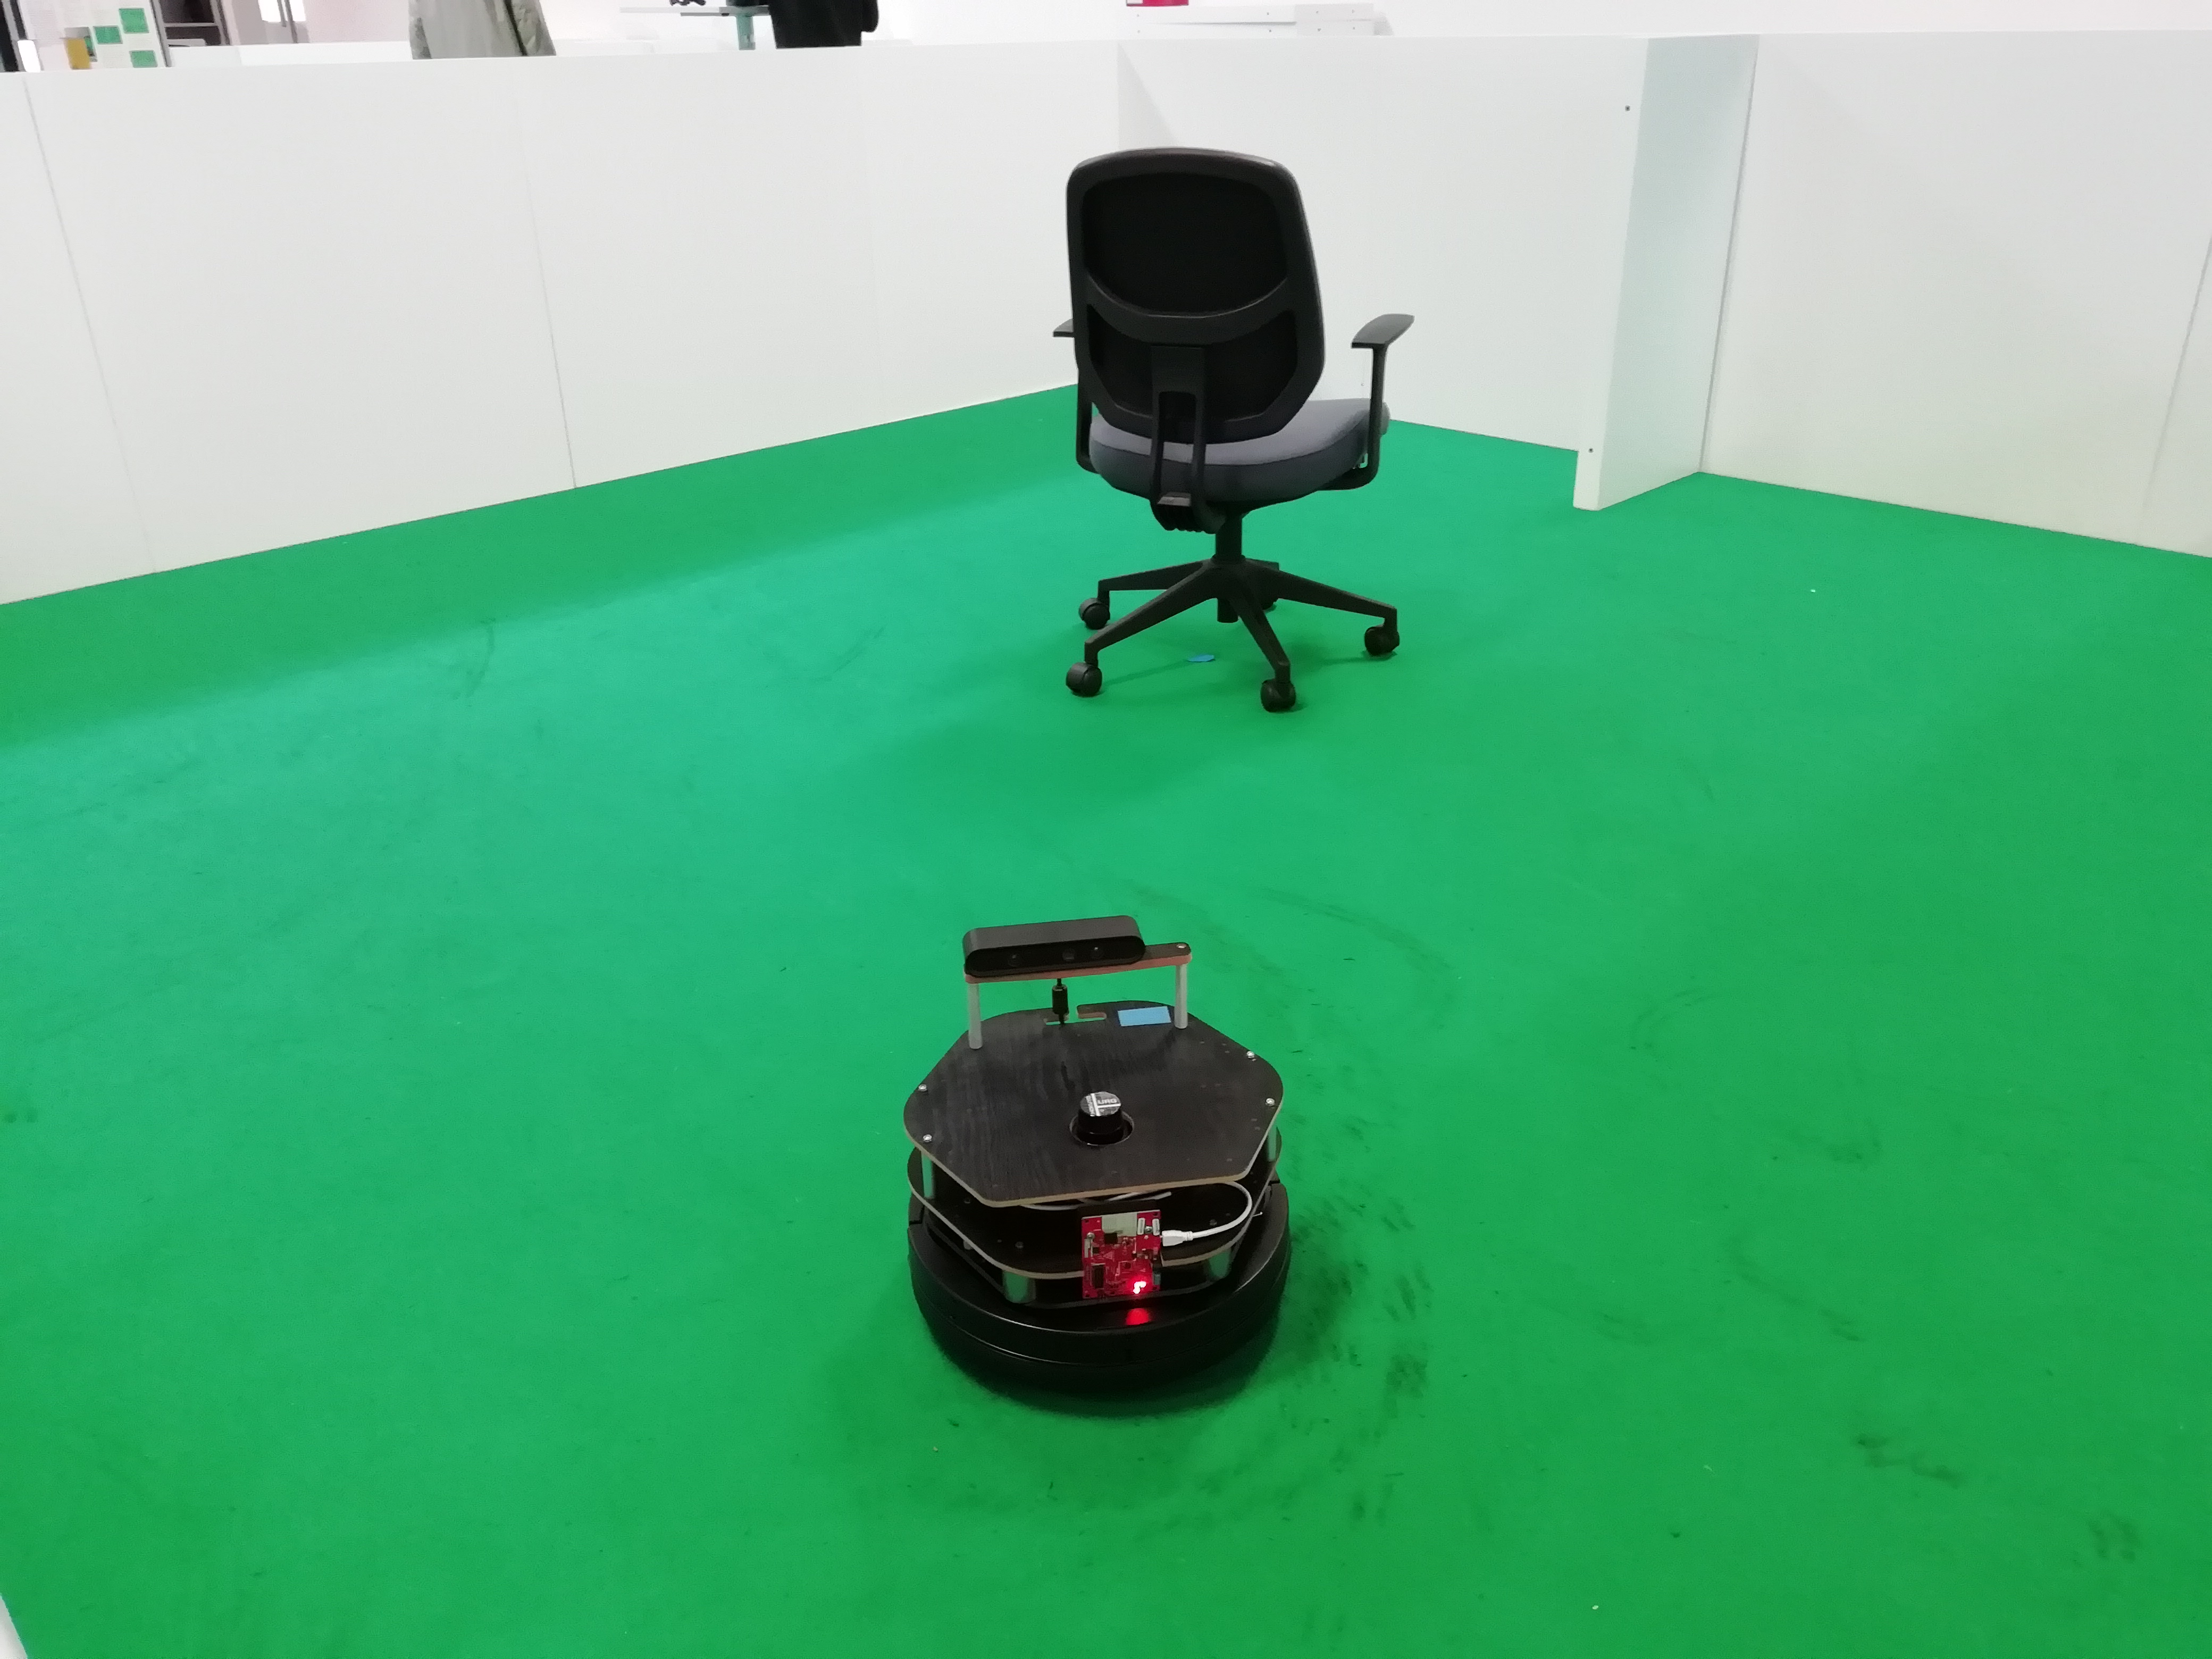
\includegraphics[width=\linewidth]{imgs/chapter5/wchair.jpg}
     \caption{Wheeled office chair}
     \label{fig::wchair}
  \end{subfigure}
  \begin{subfigure}[b]{0.3\linewidth}
    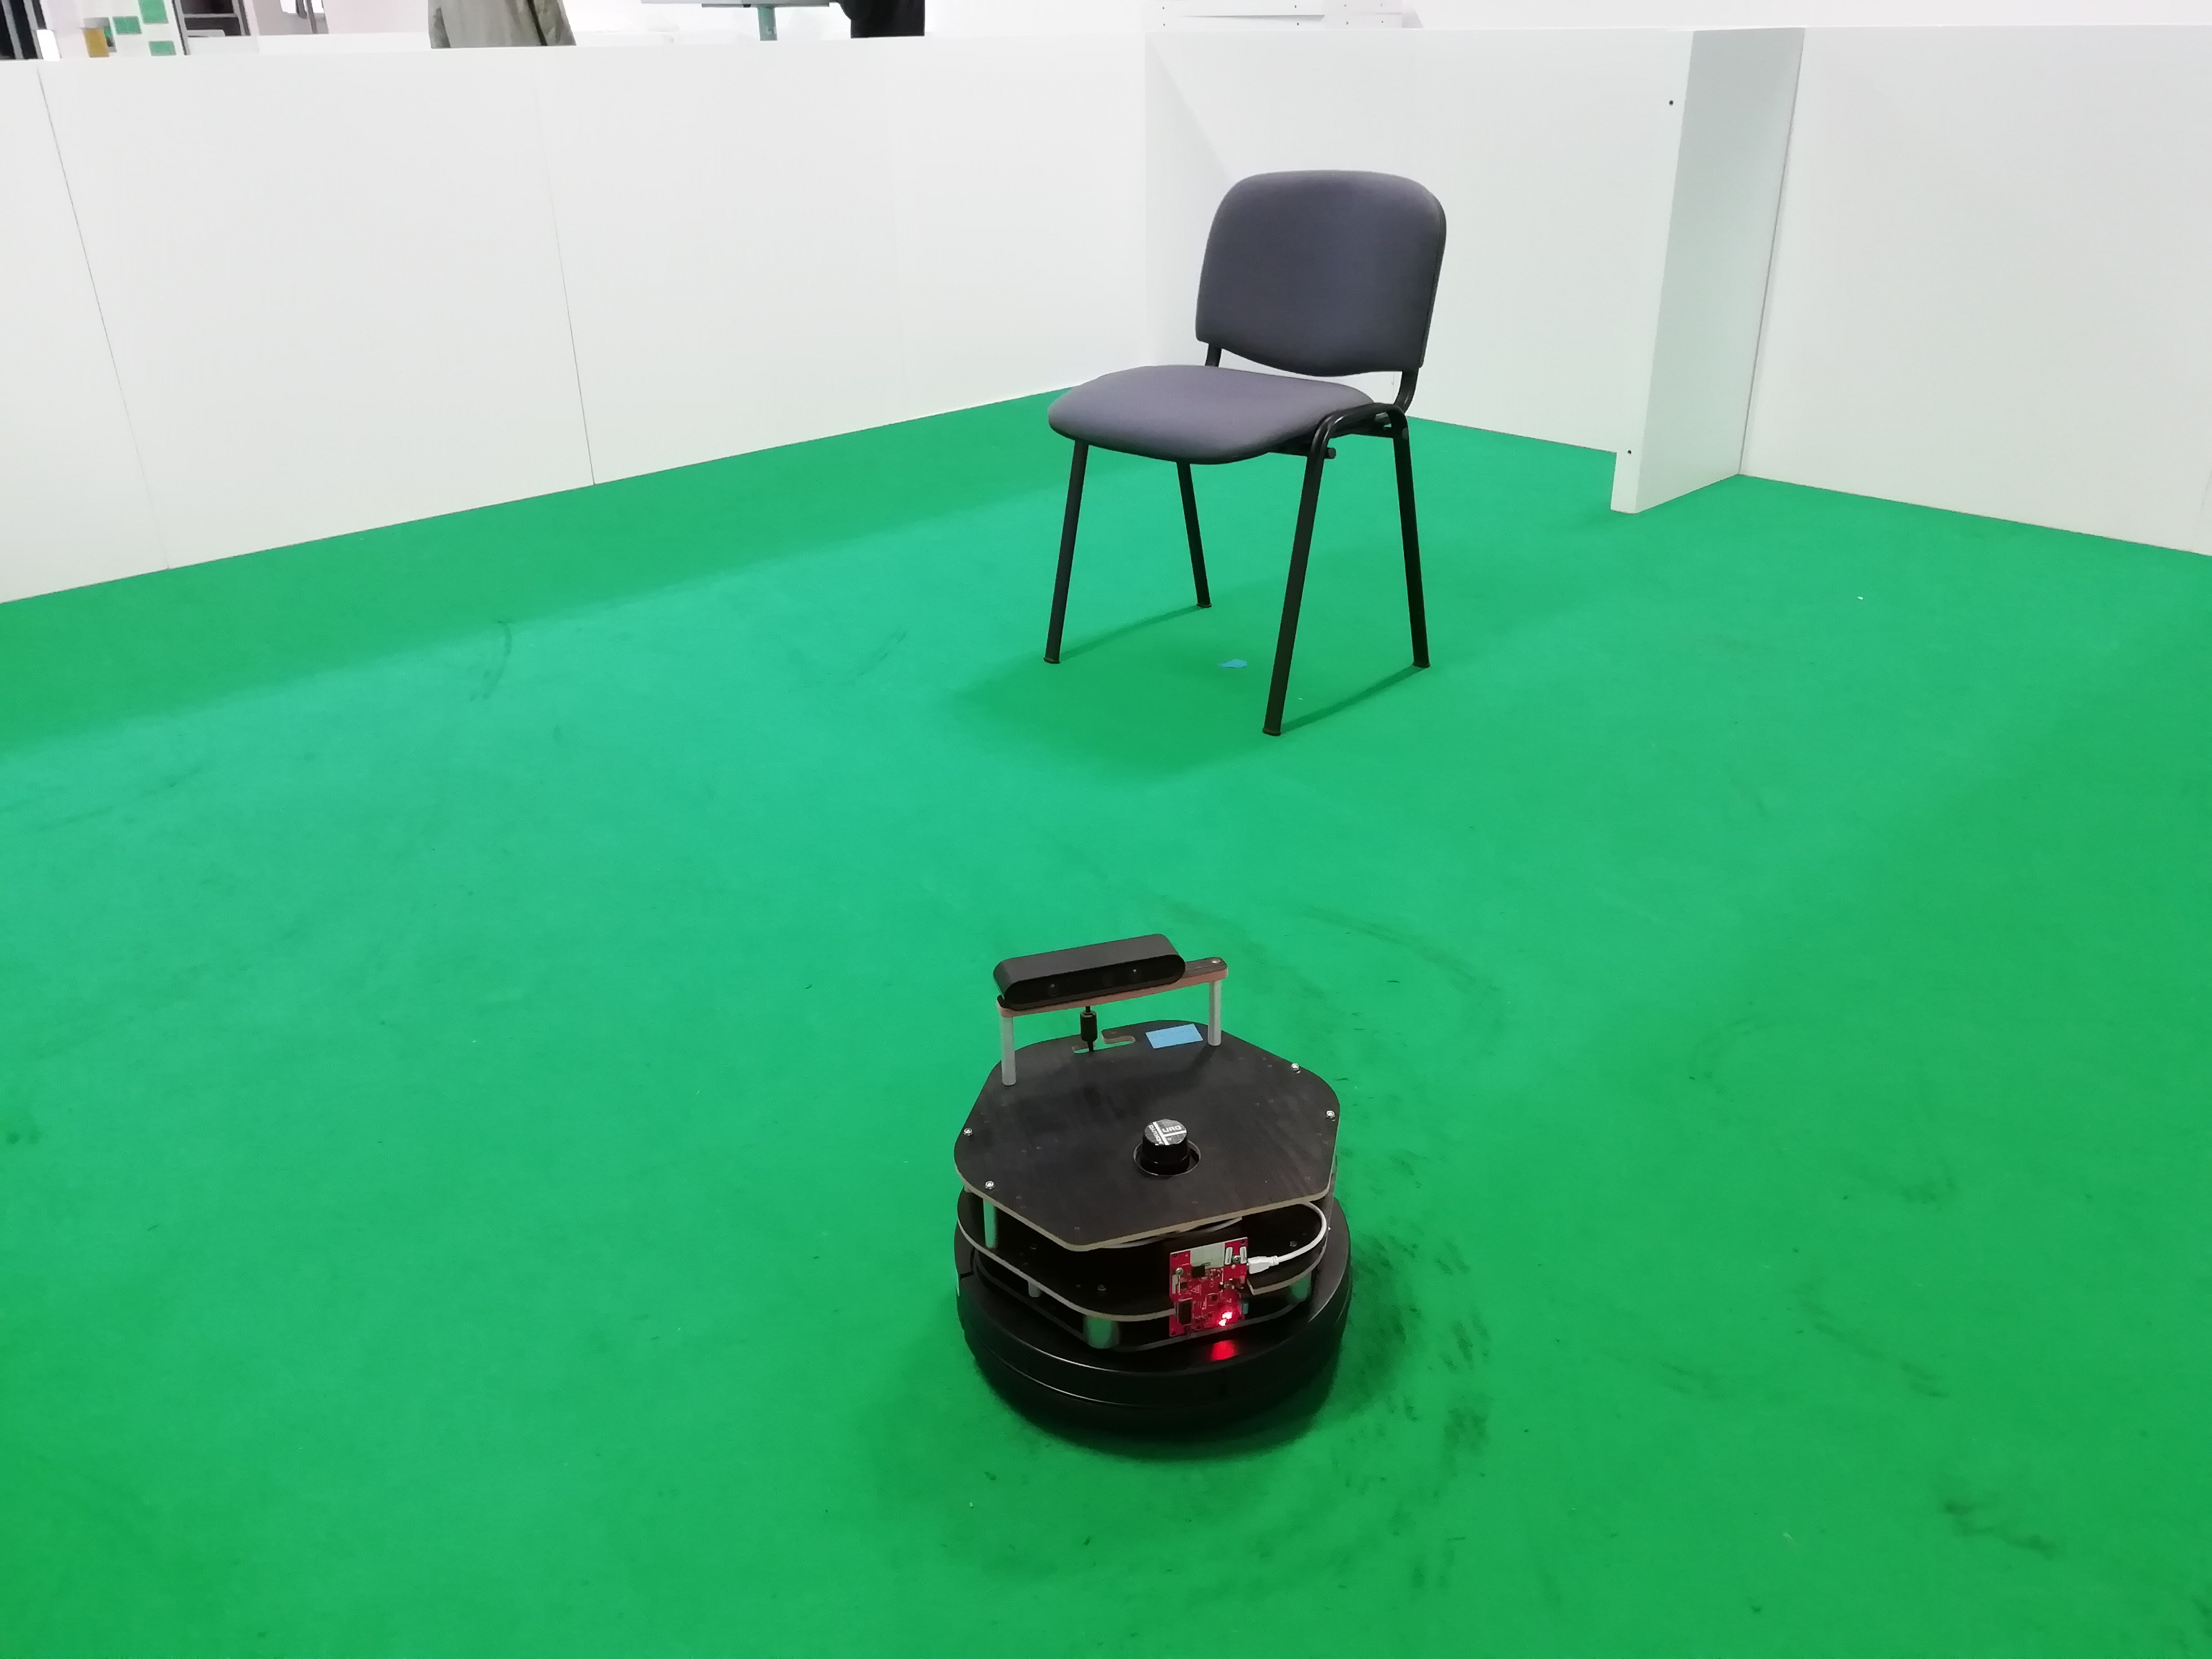
\includegraphics[width=\linewidth]{imgs/chapter5/nchair.jpg}
    \caption{Four legged chair}
    \label{fig::nchair}
  \end{subfigure}
  \begin{subfigure}[b]{0.3\linewidth}
    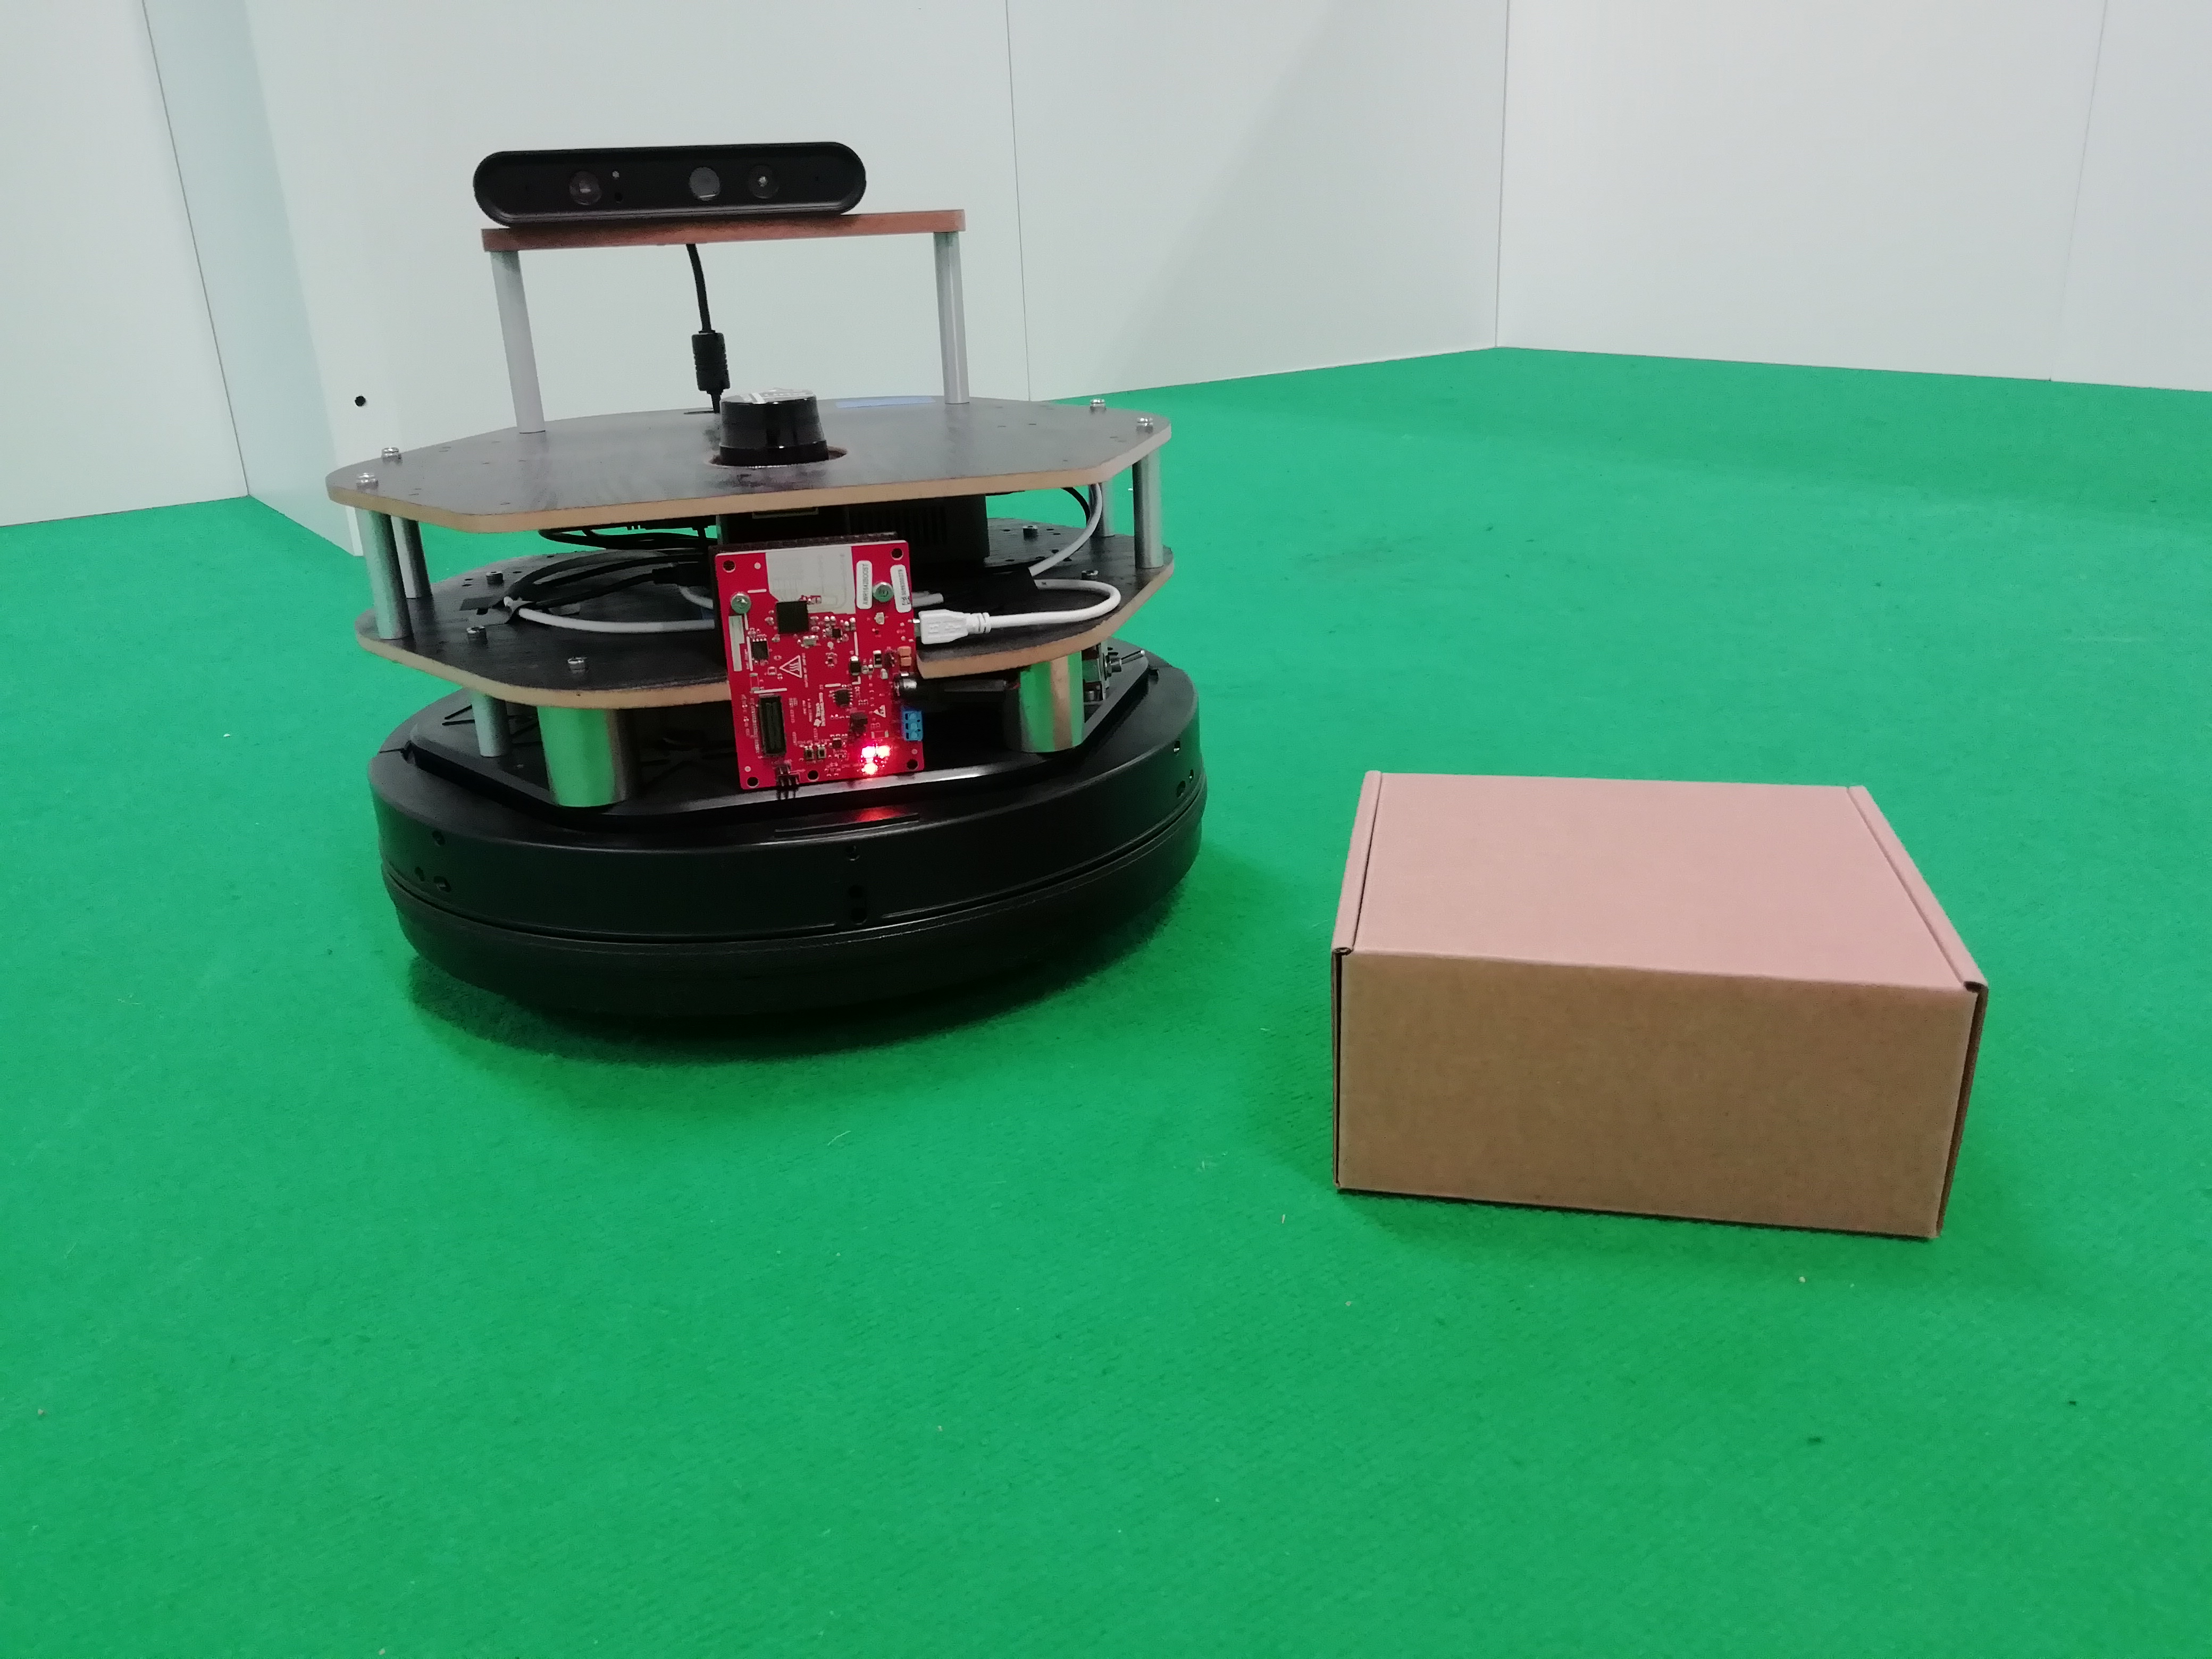
\includegraphics[width=\linewidth]{imgs/chapter5/box.jpg}
    \caption{Low height box}
    \label{fig::box}
  \end{subfigure}
  \begin{subfigure}[b]{0.3\linewidth}
    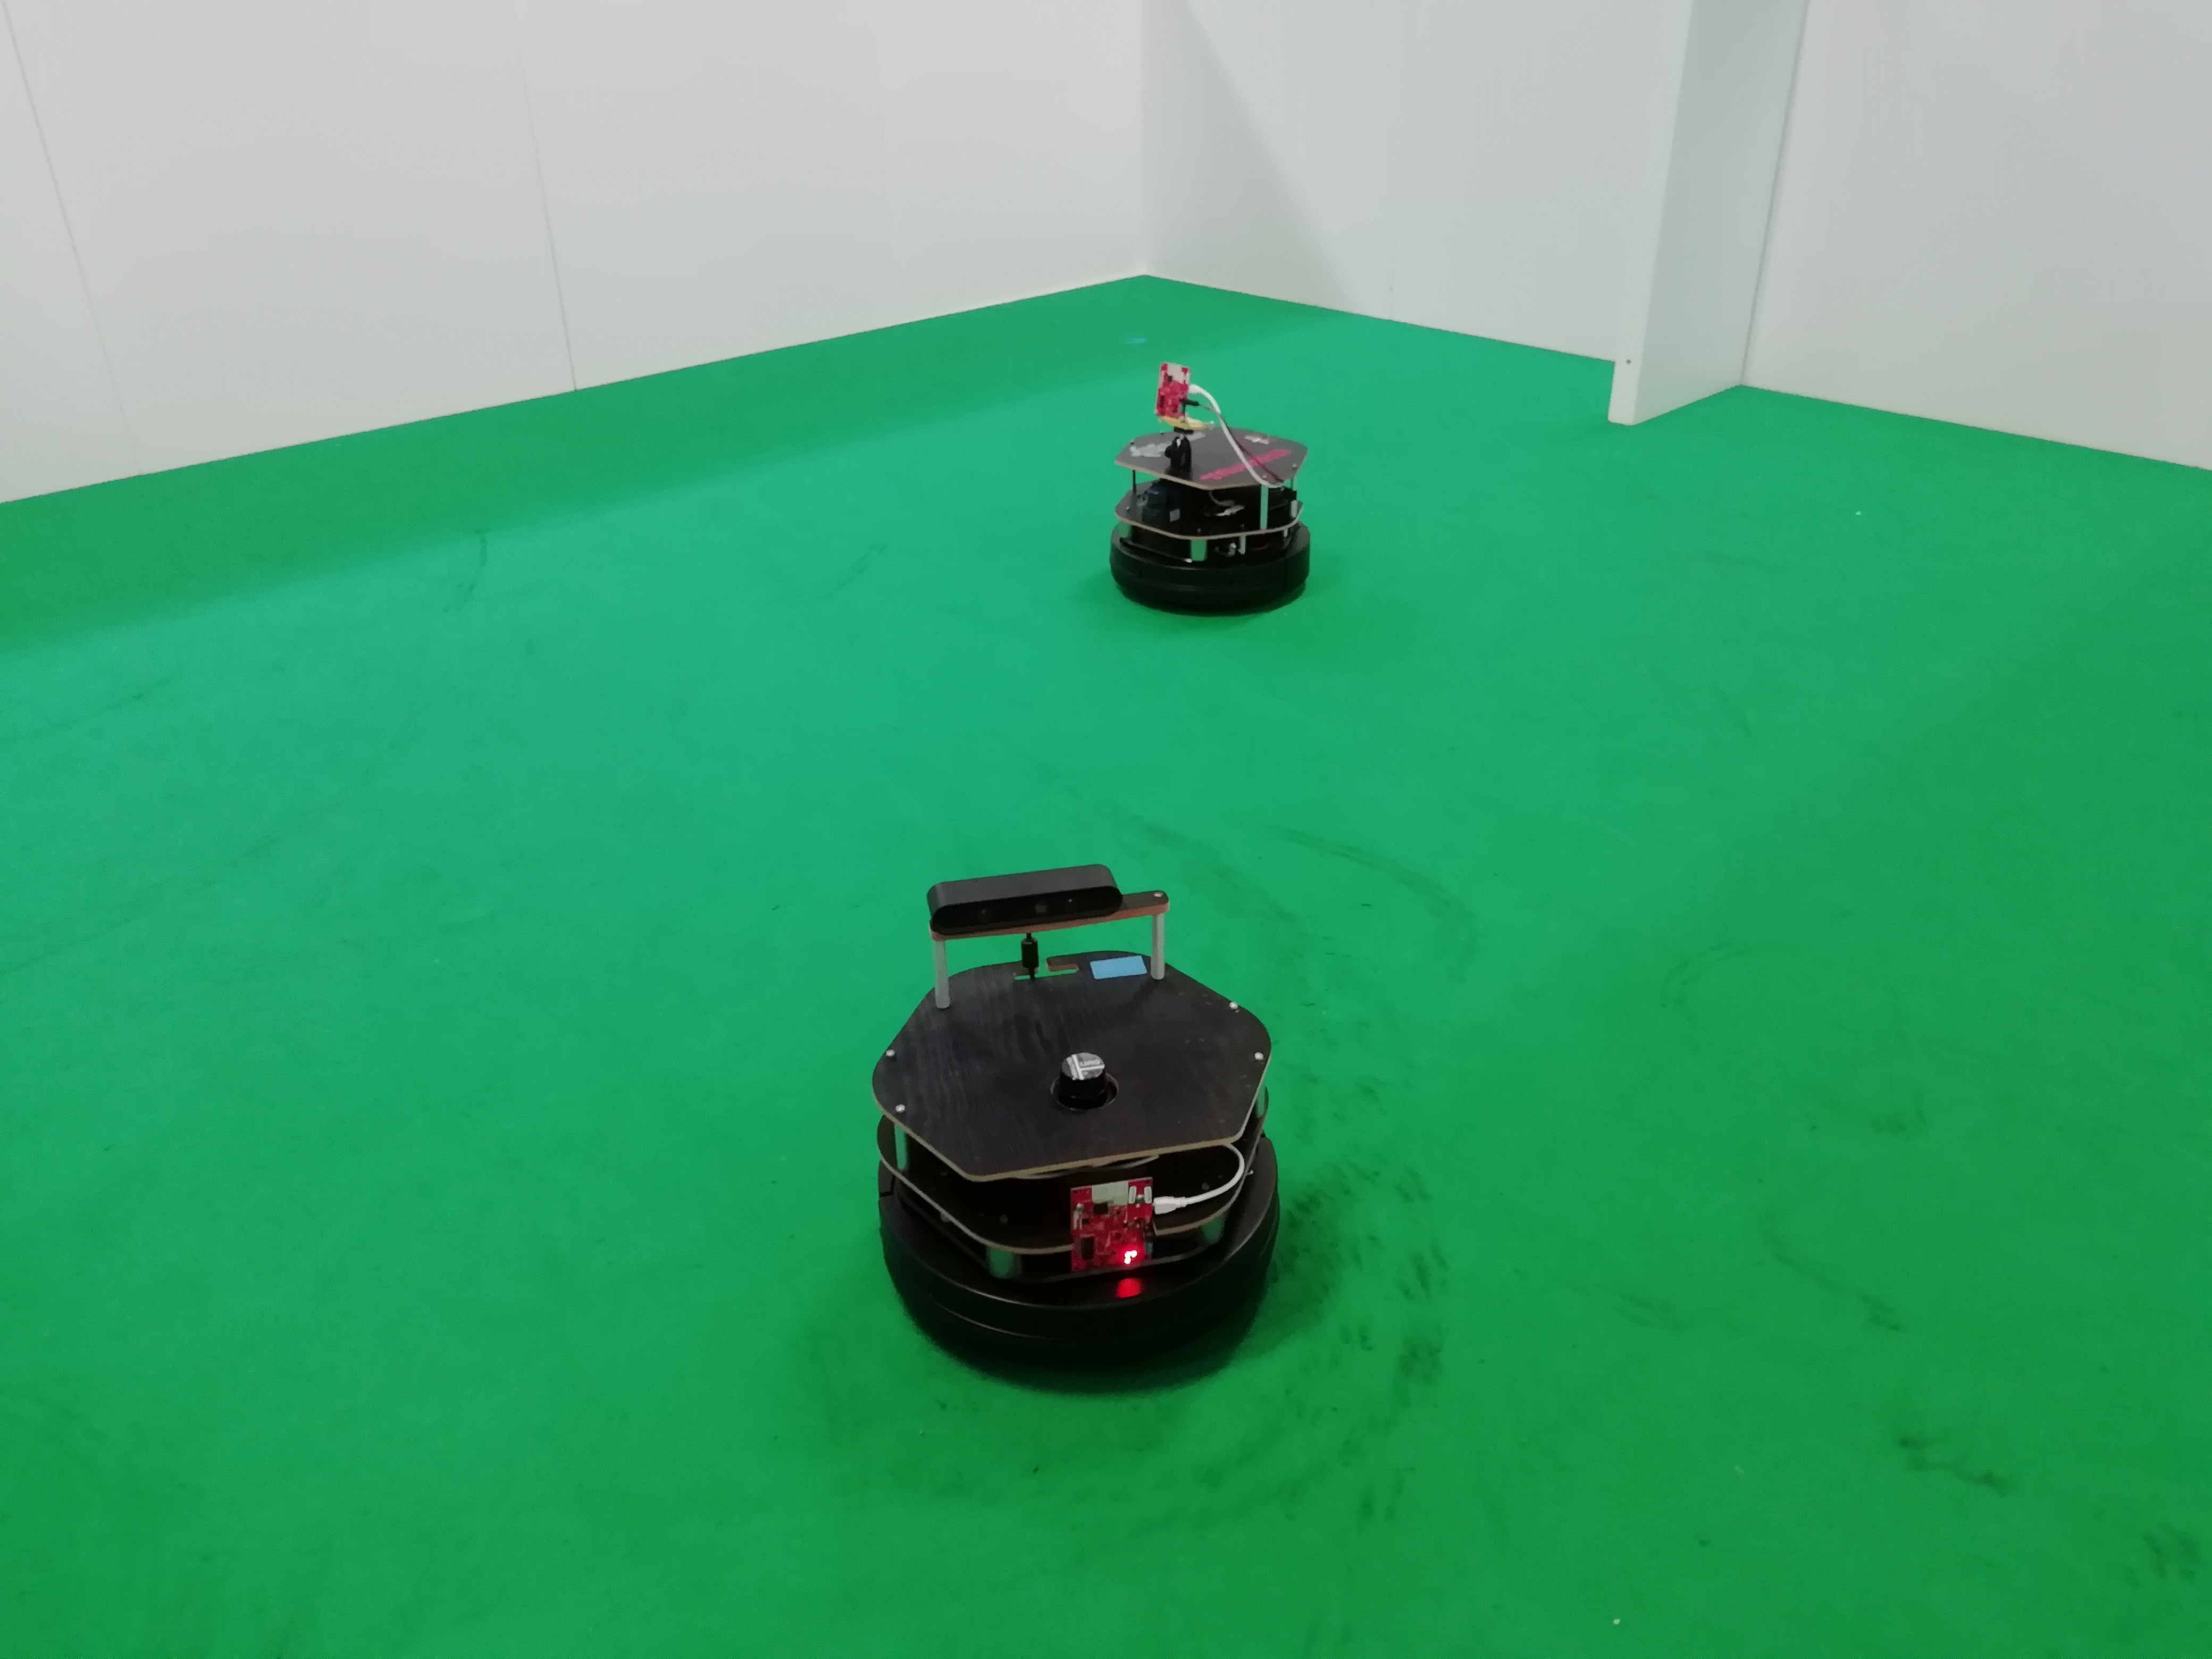
\includegraphics[width=\linewidth]{imgs/chapter5/robot.jpg}
    \caption{Another turtlebot}
    \label{fig::robot}
  \end{subfigure}
  \begin{subfigure}[b]{0.3\linewidth}
    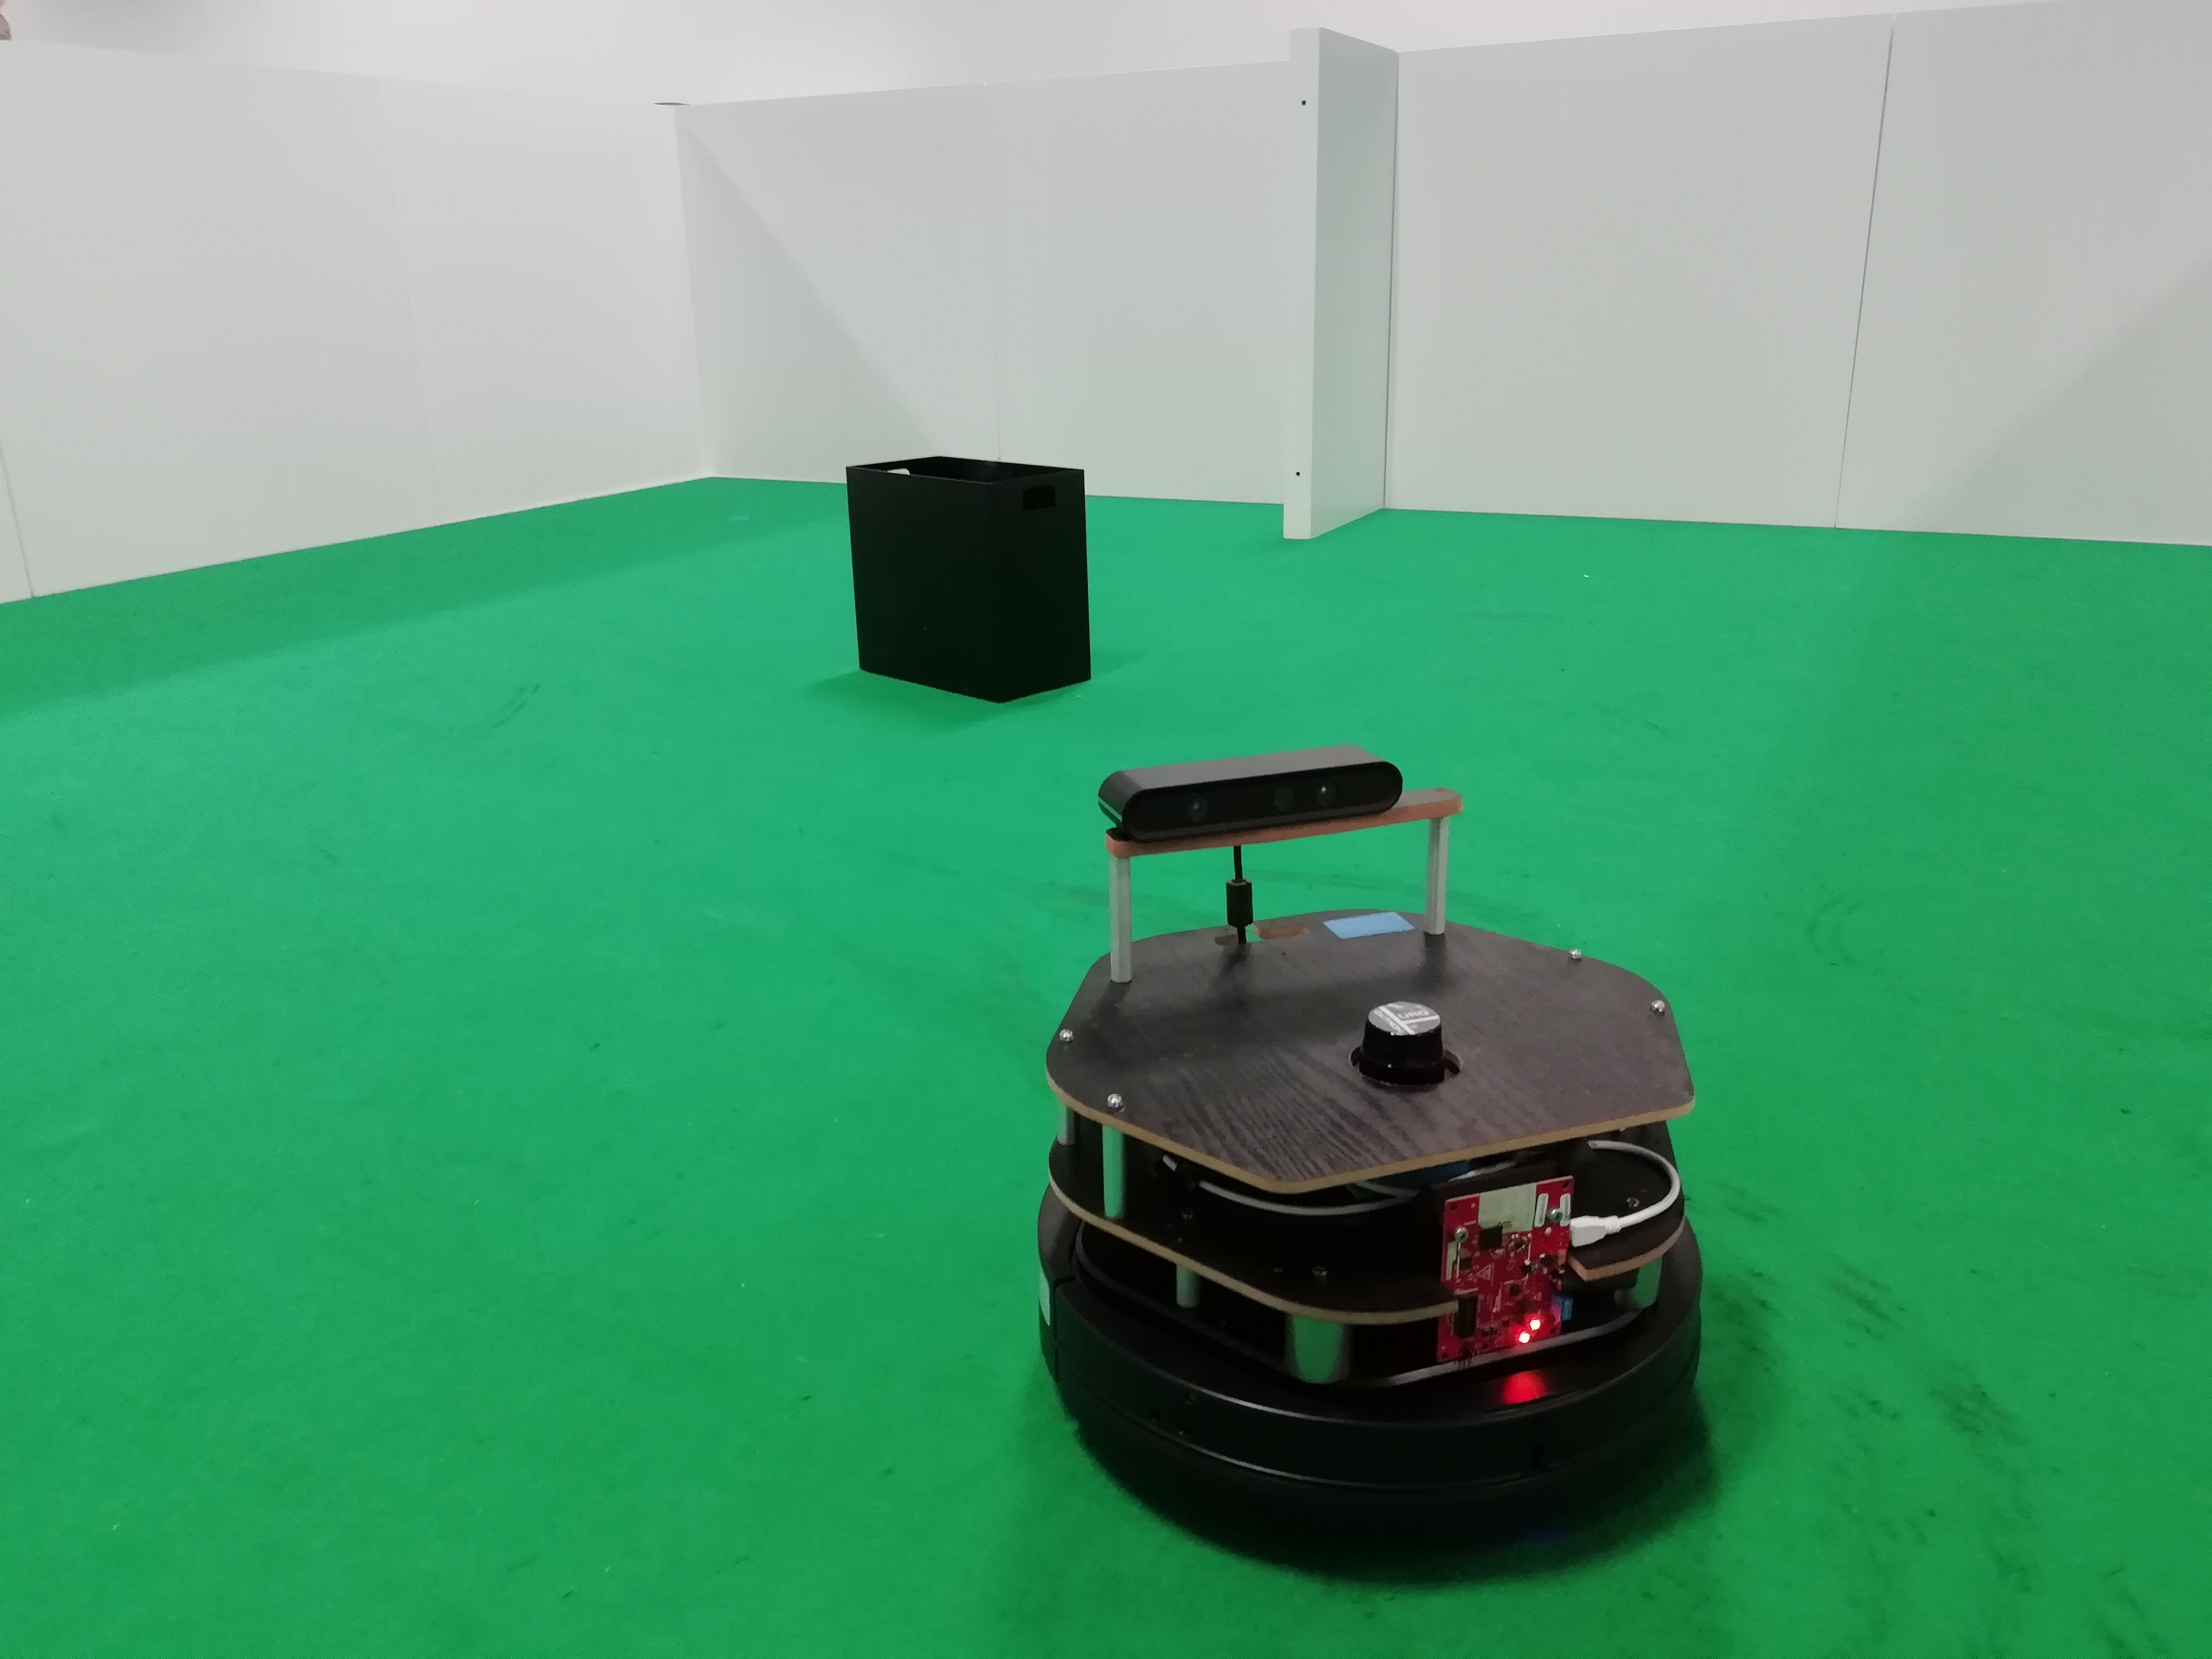
\includegraphics[width=\linewidth]{imgs/chapter5/garbage.jpg}
    \caption{Garbage Bin}
    \label{fig::garbage}
  \end{subfigure}
  \begin{subfigure}[b]{0.3\linewidth}
    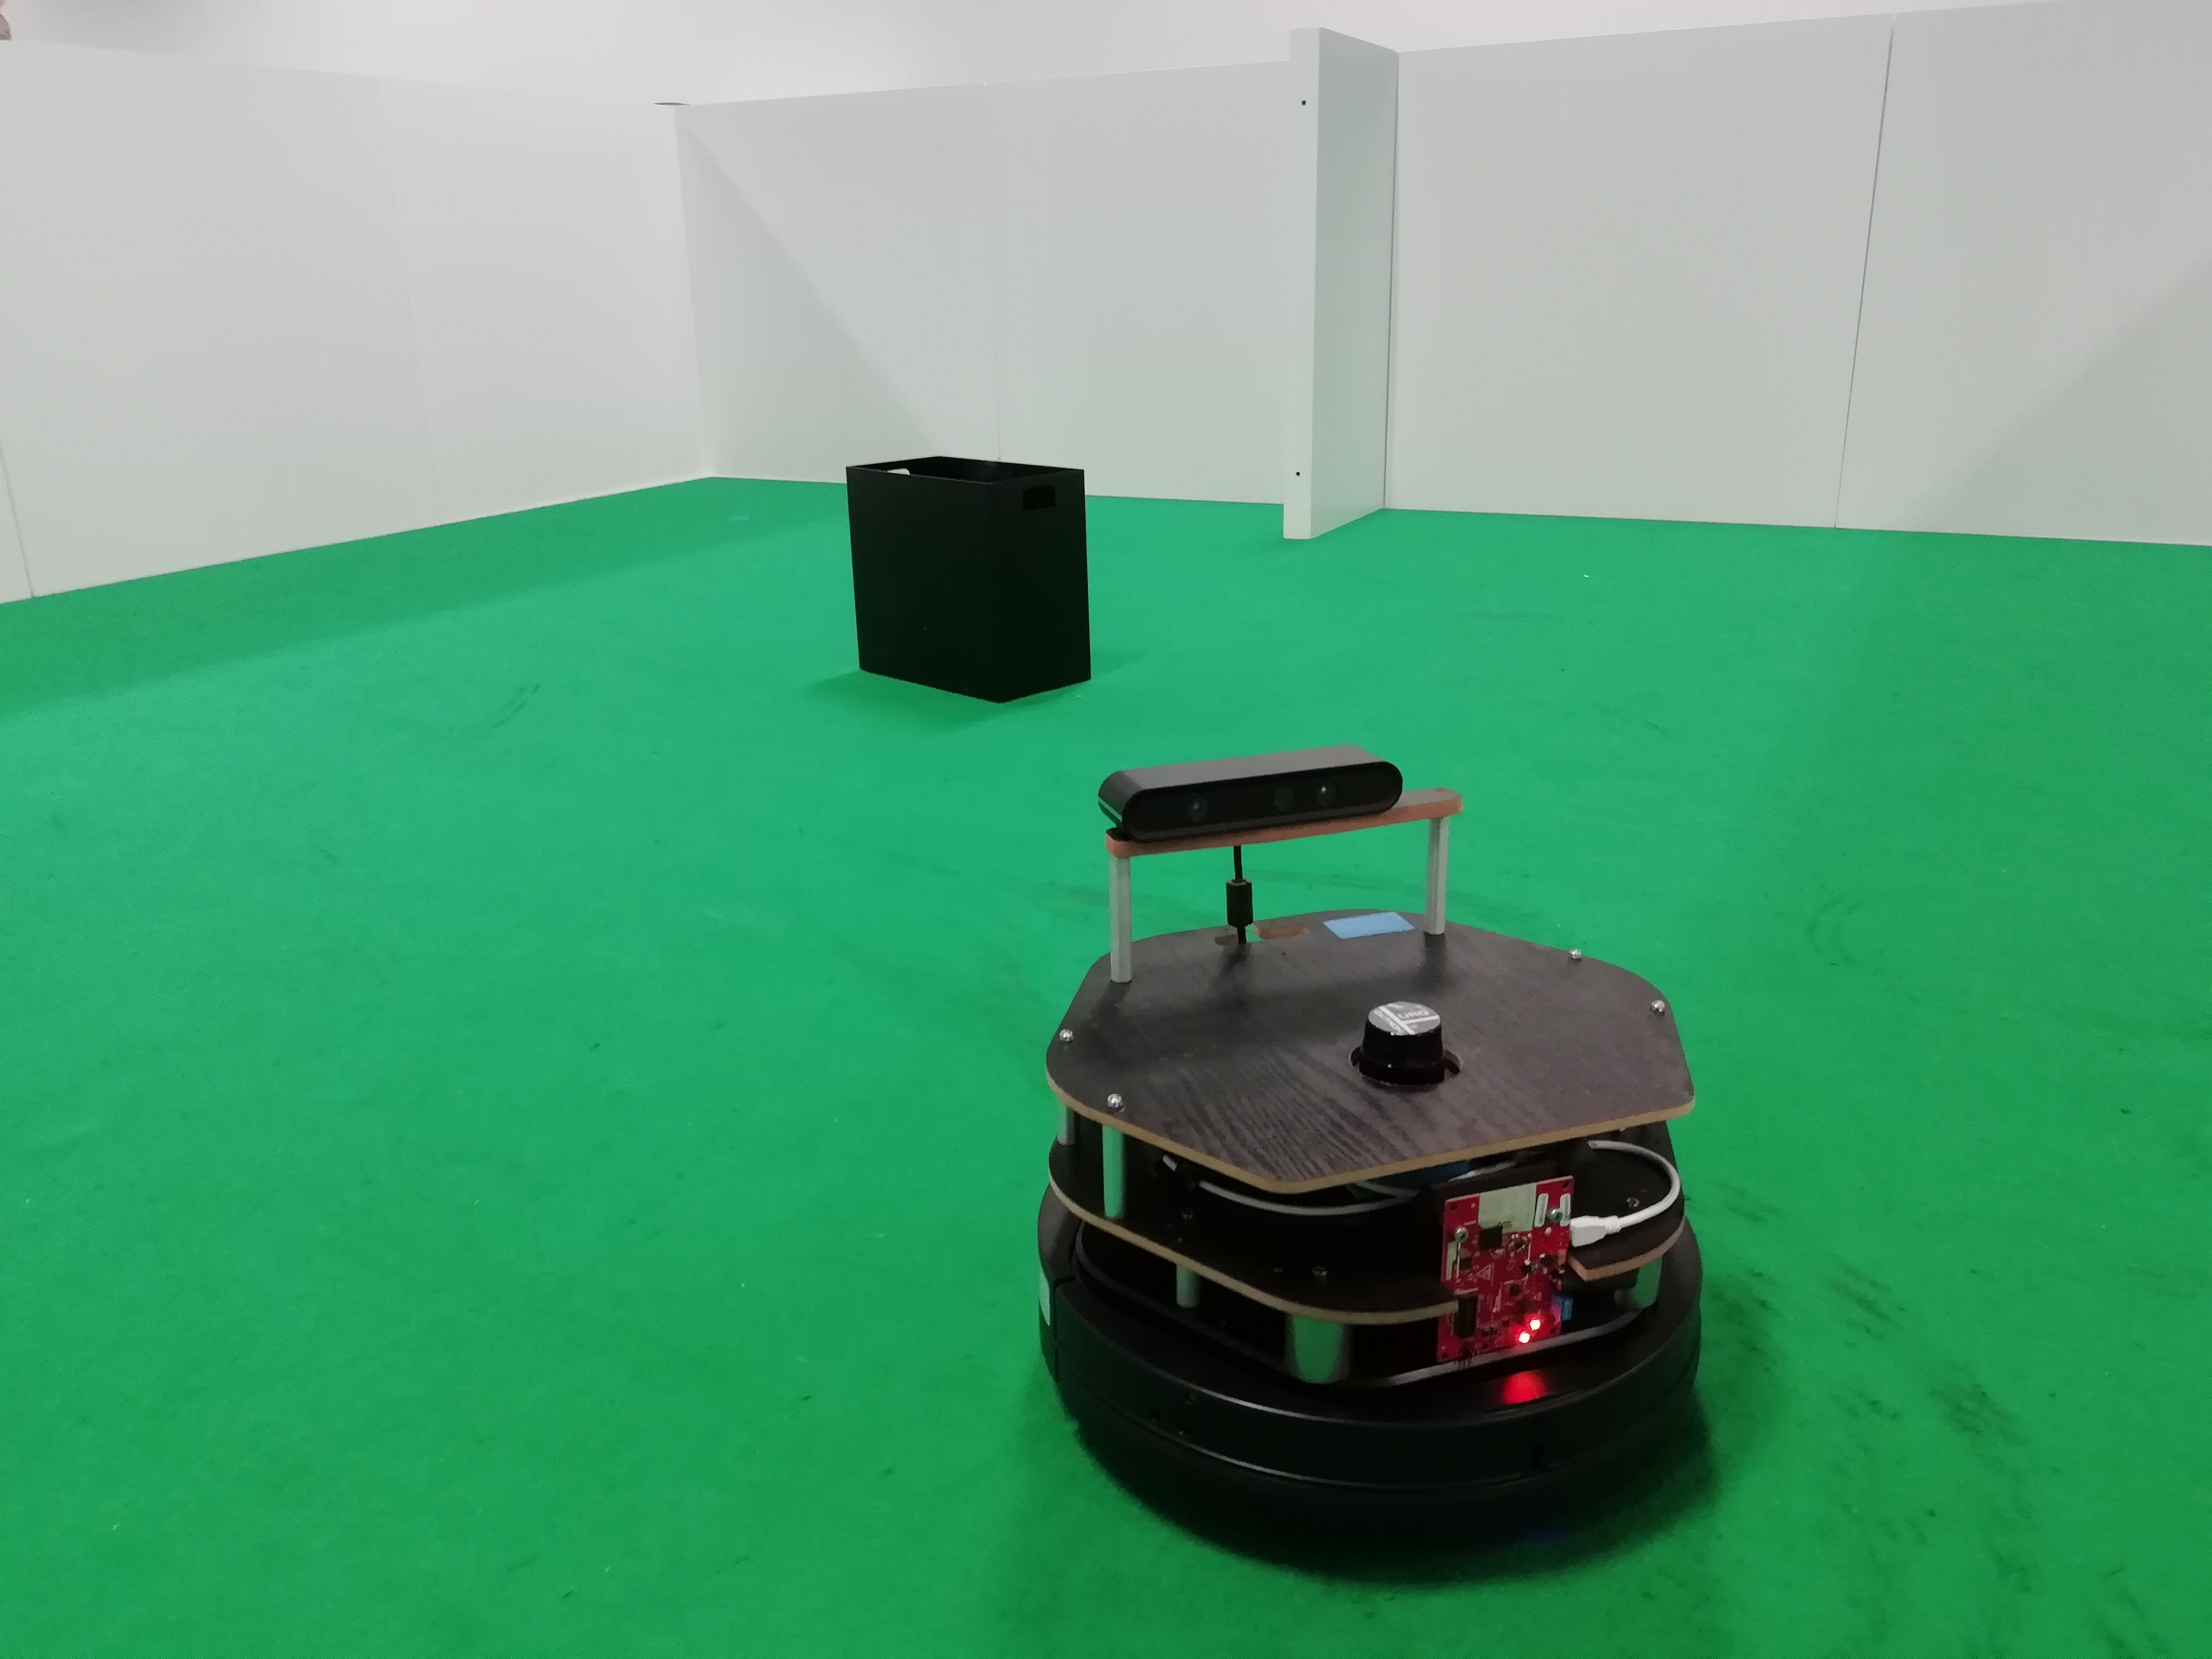
\includegraphics[width=\linewidth]{imgs/chapter5/garbage.jpg}
    \caption{Garbage Bin}
    \label{fig::garbage}
  \end{subfigure}
  \caption{Different obstacles used for the controlled test}
  \label{fig:obstacles}
\end{figure}
%LIST


\subsection{Results}
In this section we show the results of how the robot performed in avoiding the previous obstacles using different type of sensor sources (\ac{FMCW} radar, the 2D \ac{LiDAR} and both).

\subsubsection{Office Chair}
\begin{figure}
\centerline{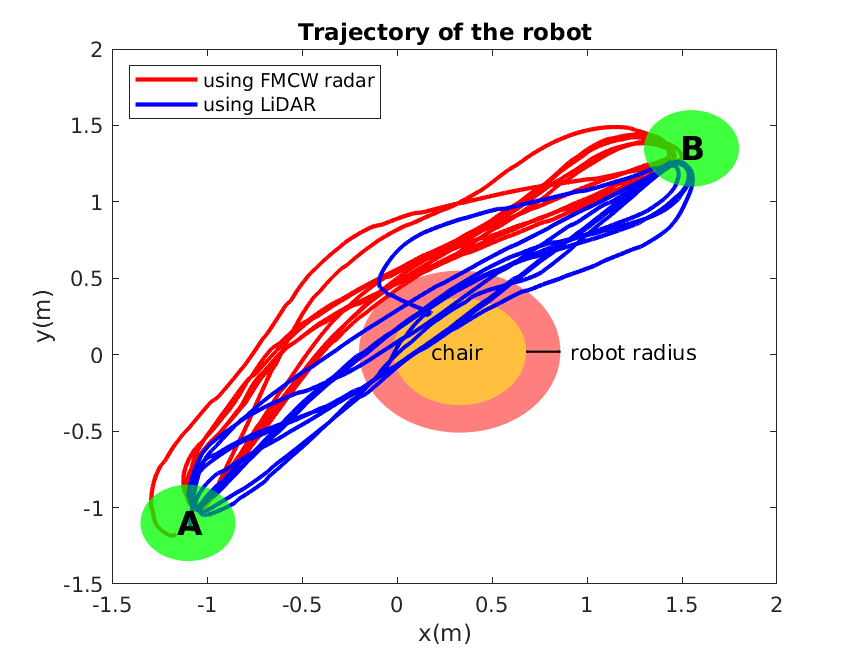
\includegraphics [width=0.7 \textwidth]{imgs/chapter5/traj1.png}}
\caption{Trajectory of the robot for the wheeled chair's case}
\label{fig:turlebot2}
\end{figure}

In the \ac{LiDAR}'s case  the robot completely disregarded the chair going in a straight line and pushing it until it was away from the experimental setup has shown in the video X. This was due to the 2D \ac{LiDAR} only detecting the leg of the chair and not the wheels. This means that the robot only perceived a single point as being occupied and not the full area of the chair. Although the inflation layer  might correct this error in some cases, since the detection is so late the robot still is unable to avoid it.

However with the \ac{FMCW} radar the chair is detected almost immediately, this makes the global planner and motion controller to be able to adjust in a very comfortable way and with it the robot is able to avoid collision. Figure X shows some instances of the first experiment. Although the detected space that the chair is occupying has some mismatch, the early detection makes up for it. However since the radar has small field of view (120 degrees) the robot might not detect the obstacle when it is passing by it which in this case lead to it scraping by the chair one time.
\subsubsection{Normal Chair}
\begin{figure}
\centerline{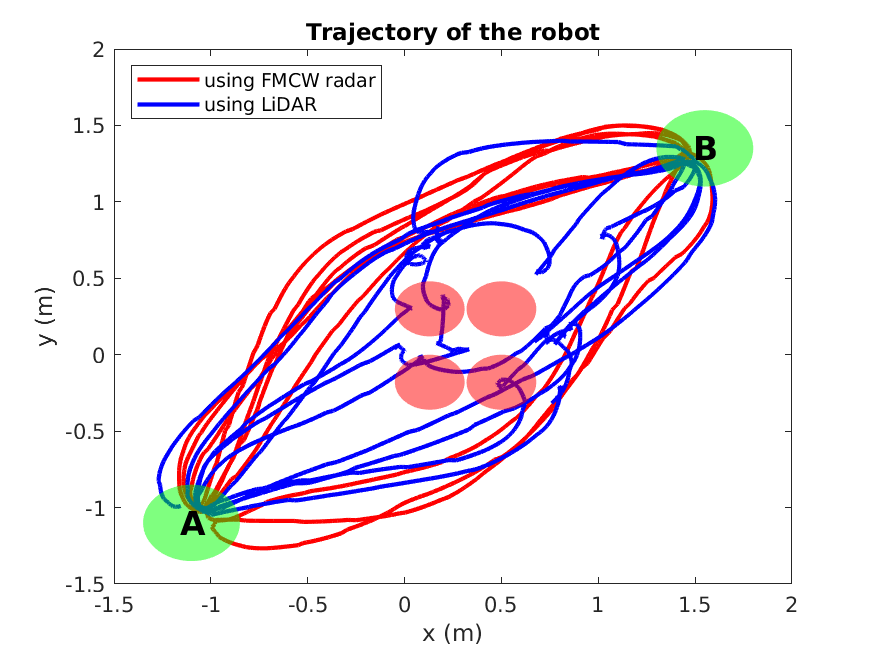
\includegraphics [width=0.7 \textwidth]{imgs/chapter5/traj2.png}}
\caption{Trajectory of the robot for the 4 legged chair's case}
\label{fig:turlebot2}
\end{figure}
As shown in figure X and in video y the robot did not perform optimally using \ac{LiDAR}. First off it went in a straight line just as the previous case almost hitting  the legs of the chair. However when it got to close to it, it came to a halt and kept oscillating for a long time until it either collided with the leg or scrapping by it. This was again due to the \ac{LiDAR} only detecting the obstacles at small distances. This behavior repeated itself throughout the task, leading to the chair being pushed several times. 

Using the \ac{FMCW} radar proved to be much better with the robot safely circumventing around the chair with safe distance for all duration of the task. Analysing the data we see that when the robot is facing it it detects almost all legs immediately (Fig X). This makes it so the robot is aware of it at all times and planning around it.
\begin{figure}[h] 
\centerline{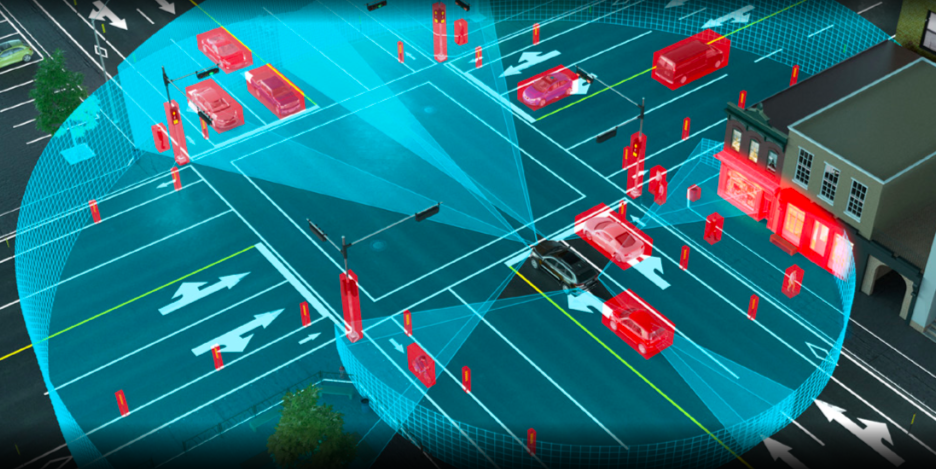
\includegraphics [width=0.7 \textwidth]{imgs/chapter/lidarcar.png}}
\caption{Trajectory of the robot using the office chair as an obstacle}
\label{fig:lidarcar}
\end{figure}

\subsubsection{Garbage Bin}
The robot went in a straight line as in the wheeled chair's case pushing the garbage bin until it reached its first goal. This happened again because the \ac{LiDAR} was unable to detect the garbage bin. Using the \ac{FMCW} radar the robot did detect it properly and went around it easily.
\subsubsection{Box}
Collided with the chairs multiple times and 
\subsubsection{Robot}
Both \ac{LiDAR} and the FMCW radar were able to avoid the robot. 
In the wheeled chairs case the robot was able to detect 
- Image of plots
- explain what happened
- explain some navigation stack stuff

\section {Experiment 4}